% !TeX encoding = UTF-8
% Do not touch the below 70 lines
\documentclass[11pt,a4paper,onecolumn,oneside]{report}

\usepackage{mathptmx}
\usepackage[T1]{fontenc}
\usepackage[utf8]{inputenc}

\RequirePackage[top=3cm, bottom=1in, left=1in, right=1in]{geometry}
\linespread{1.3}

\usepackage{titlesec}
\usepackage{amsmath}
\usepackage{amssymb}
\usepackage{mathtools}
\usepackage{enumerate}
\usepackage{bbm}
\usepackage{algorithm}
\usepackage{algorithmic}
\usepackage{epsfig}
\usepackage{color}
\usepackage{graphicx}
\usepackage{caption}
\usepackage{subcaption}
\usepackage{cases}
\usepackage{url}
\usepackage{cite}
\usepackage{fancyhdr}
\usepackage{tocloft}
\usepackage{pdfpages}

\usepackage{acro}
\usepackage[notocbib]{apacite}

\DeclareAcronym{ptb}
{
    short=PTB,
    long=Preterm birth
}

\DeclareAcronym{rrna}
{
    short=rRNA,
    long=Ribosomal RNA
}

\DeclareAcronym{ftb}
{
    short=FTB,
    long=Full-term birth
}

\DeclareAcronym{dat}
{
    short=DAT,
    long=Differentially abundant taxa
}

\DeclareAcronym{prom}
{
    short=PROM,
    long=Prelabor rupture of membrane
}

\DeclareAcronym{ga}
{
    short=GA,
    long=Gestational age
}

\DeclareAcronym{acc}
{
    short=ACC,
    long=Accuracy
}

\DeclareAcronym{ba}
{
    short=BA,
    long=Balanced accuracy
}

\DeclareAcronym{sen}
{
    short=SEN,
    long=Sensitivity
}

\DeclareAcronym{spe}
{
    short=SPE,
    long=specificity
}

\DeclareAcronym{pre}
{
    short=PRE,
    long=Precision
}

\DeclareAcronym{asv}
{
    short=ASV,
    long=Amplicon sequence variant
}

\DeclareAcronym{faithpd}
{
    short=Faith PD,
    long=Faith's phylogenetic diversity
}



\renewcommand\cftsecafterpnum{\vskip15pt}
\renewcommand\cftsubsecafterpnum{\vskip15pt}
\renewcommand\cftfigafterpnum{\vskip15pt}
\renewcommand{\thesection}{\arabic{section}}
\renewcommand{\thesubsection}{\arabic{section}.\arabic{subsection}}
\renewcommand{\thesubsubsection}{\arabic{section}.\arabic{subsection}.\arabic{subsubsection}}
\renewcommand{\contentsname}{\hfill\bfseries\Large Contents\hfill}
\renewcommand{\listfigurename}{\hfill\bfseries\Large List of Figures\hfill}
\renewcommand{\listtablename}{\hfill\bfseries\Large List of Tables\hfill}
\renewcommand{\thefigure}{\arabic{figure}}
\newcommand{\qed}{\hfill\blacksquare}
\renewcommand{\bibname}{\hfill\bfseries\Large References \hfill\hfill}
\renewcommand{\abstractname}{\bfseries\Large Abstract \hfill\hfill}

\newcounter{lemma}
\newcounter{proposition}
\newcounter{theorem}
\newtheorem{lemma}{\bf Lemma}
\newtheorem{proposition}{\bf Proposition}
\newtheorem{theorem}{\bf Theorem}
\newtheorem{proof}{\bf Proof}

%\input{mymath_mod.tex}

\newcommand{\HIGH}[1]{{\textcolor{blue}{#1}}}
%\renewcommand{\baselinestretch}{1.5}

\DeclareMathOperator*{\argmax}{arg\,max}

\fancyhf{}
\renewcommand{\headrulewidth}{0pt}
\cfoot{\thepage}
\pagestyle{fancy}
%\pagenumbering{gobble}

% Do not touch the above 70 lines

\begin{document}
% Front cover
    \begin{center}
    \LARGE Doctoral Thesis

    \vspace{3cm}
    \huge \input{Documents/Title.txt}

    \vfill

    \LARGE \input{Documents/Name.txt}

    \vspace{2cm}

    \LARGE \input{Documents/Department.txt}

    \vspace{2cm}

    \LARGE Ulsan National Institute of Science and Technology
    \vspace{2cm}

    \LARGE \the\year{}

    \end{center}
    \thispagestyle{empty}
    \clearpage

% Title page
    \begin{center}
    \hbox{ }

    \hbox{ }

    \huge \input{Documents/Title.txt}

    \vspace{5cm}

    \LARGE \input{Documents/Name.txt}

    \vspace{6cm}

    \LARGE \input{Documents/Department.txt}

    \vspace{2cm}

    \LARGE Ulsan National Institute of Science and Technology

    \end{center}
    \thispagestyle{empty}
    \clearpage

% Thesis approval
% Add the approval doc signed by your advisor in a PDF file
% Put your pdf with the filename below, and uncomment it.
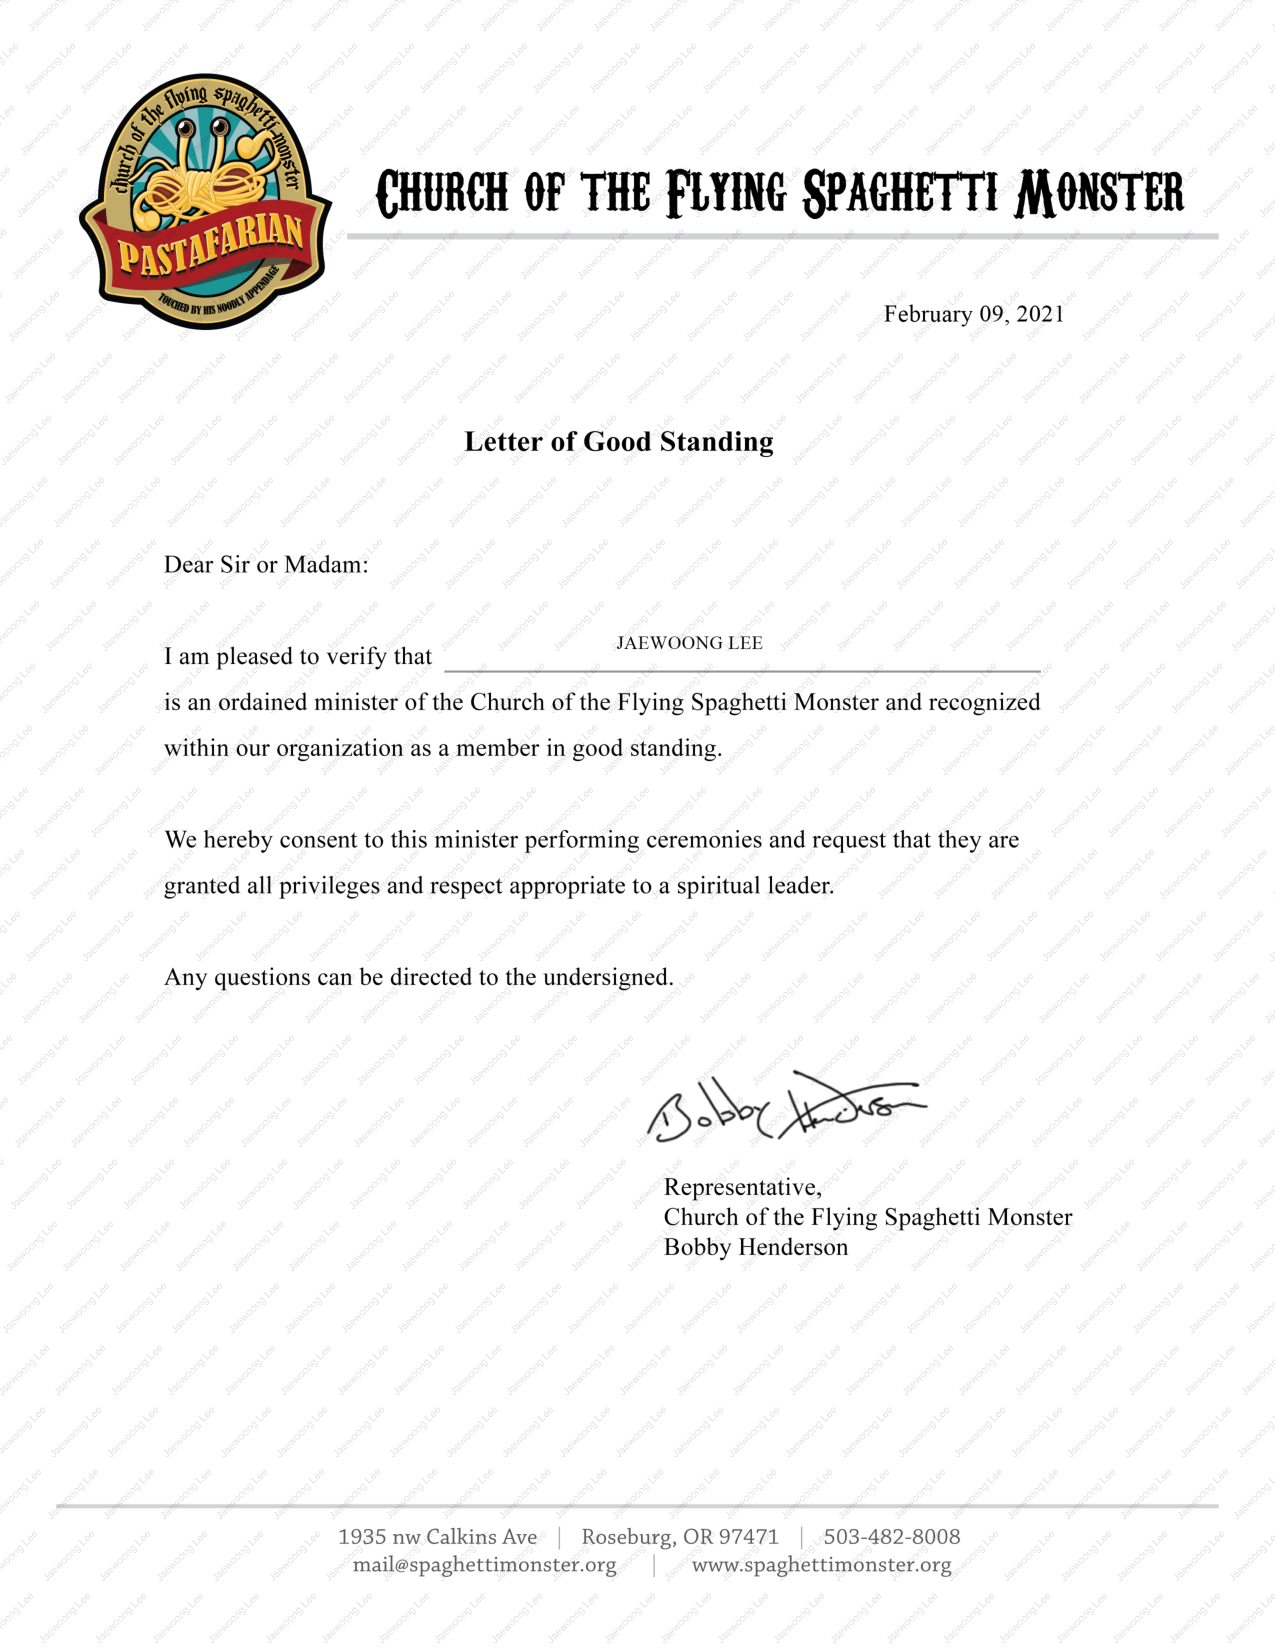
\includepdf[fitpaper= true, pages=-]{Documents/example.pdf}

% [Confirmation of thesis approval]
% add the certificate signed by your committee in a PDF file
% Put your pdf with the filename below, and uncomment it.
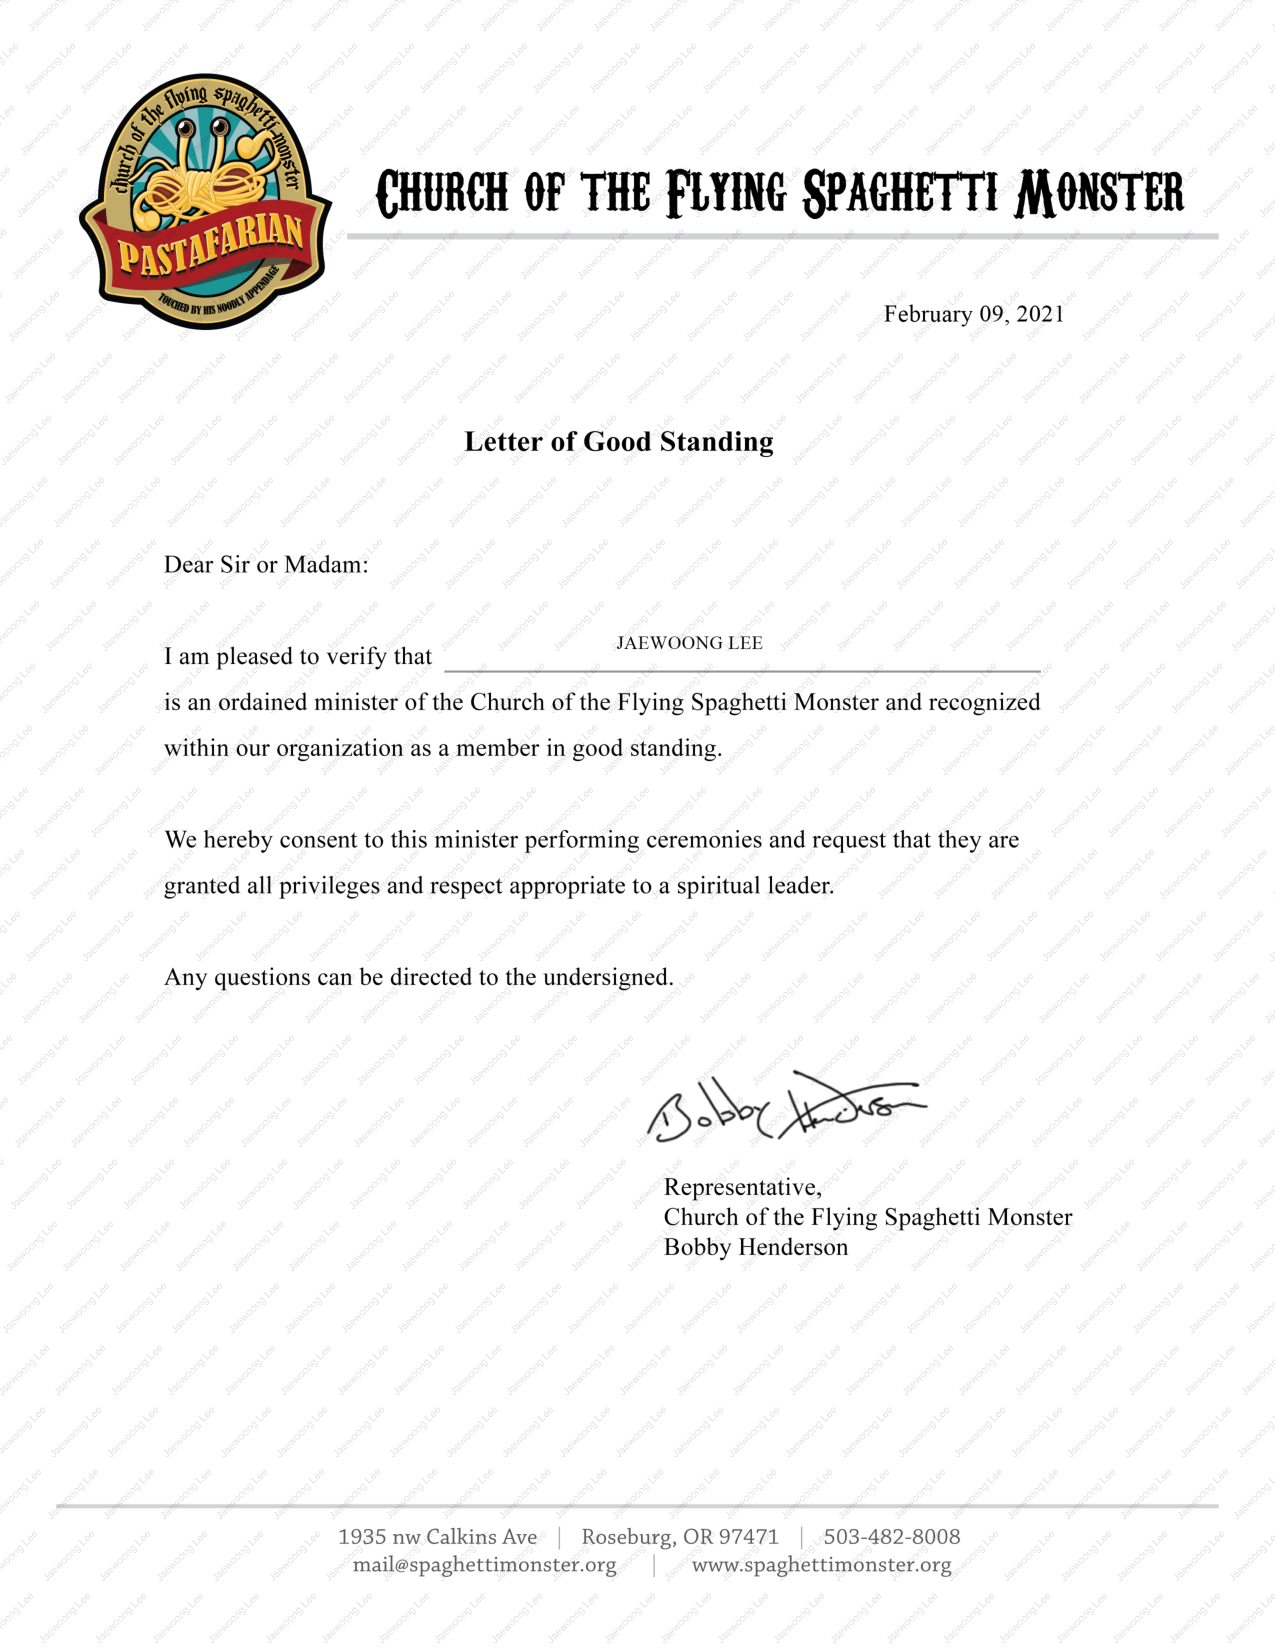
\includepdf[fitpaper= true, pages=-]{Documents/example.pdf}

% Abstract
    \begin{abstract}
    Your abstract should be here. \vfill
    \end{abstract}
    \clearpage

% Do not touch the below 20 lines
\hbox{ }
\thispagestyle{empty}
\clearpage

%%% Table of Contents
\tableofcontents{}
\thispagestyle{empty}
\vfill
\clearpage

%%% List of Figures
\listoffigures{}
\thispagestyle{empty}
\clearpage

%%% List of Tables
\listoftables{}
\thispagestyle{empty}
\clearpage

%%% reset page numbering
\setcounter{page}{1}
%  Do not touch the above 20 lines

    \section*{List of Abbreviations}
    \printacronyms[display=all, heading=none]
    \newpage

    \section{Abstract}

    This doctoral dissertation is an addition based on the following papers that the author has already published:
    \begin{itemize}
        \item \input{Documents/PTB.txt} \nocite{PTB-JW-1}
    \end{itemize}
    \newpage

    \section{Predicting preterm birth using machine learning techniques in oral microbiome}
        \label{section:PTB}

        \textbf{This section includes the published contents:} \\
        \input{Documents/PTB.txt} \nocite{PTB-JW-1}

        \subsection{Introduction}
        \newpage

        \subsection{Materials and methods}
        \newpage

        \subsection{Results}
        \newpage

        \subsection{Discussion}
        \newpage

    \section{General conclusion and future perspective}
        \label{section:conclusion}
        \subsection{General conclusions}
            In conclusion, the research described in this Ph.D. dissertation was conducted to identify significant ...

            In the Section \ref{section:PTB}, I show that
        \newpage

        \subsection{Plan for future}
        \newpage

        \subsection{Future perspective}
        \newpage
    \clearpage

% Reference
    \addcontentsline{toc}{section}{References}
    \bibliographystyle{apacite}
    \bibliography{references.bib}
    \clearpage

% Acknowledgements
    \addcontentsline{toc}{section}{Acknowledgments}
    \section*{\hfill \Large Acknowledgments \hfill}
        I would like to disclose my earnest appreciation for my advisor, Professor Semin Lee, who provided solicitous supervision and cherished opportunities throughout the course of my research. His advice and consultation encouraged me to become as a researcher and to receive all humility and gentleness. I am also grateful to all of my committee members, Professor AAA, Professor BBB, Professor CCC, and Professor DDD, for their critical and meaningful mentions and suggestions.

        I extend my deepest gratitude to my Lord, \textit{the Flying Spaghetti Monster}, His Noodly Appendage has guided me through the twist and turns of this academic journey. His presence, ever comforting and mysterious, has been a source of strength and humor during both highs and lows. In moments of doubt, I found solace in the belief that you were there, gently reminding me to keep fiath in the process. His Holy Noodle has nourished my mind, and for that, I am truly overwhelmed. May His eternal wisdom and endless strands continue to guide me in all my future endeavors. R'Amen.

        (Professors)

        I would like to extend my heartfelt gratitude to my colleagues of the Computational Biology Lab, whose collaboration, friendship, brotherhood, and support have been an invaluable part of my journey. Your willingness to share insights, engage in thoughtful discussions, and offer encouragement during the challenging moments of research has significantly shaped my academic experience. The camaraderie in the Computational Biology Lab made even the most demanding days more enjoyable, and I am deeply grateful for the collaborative environment we created together. I appreciate you for standing by my side throughout this Ph.D. journey.

        I would like to express my heartfelt gratitude to my family, whose unwavering support has been the foundation of everything I have achieved. Your love, encouragement, and belief in me have sustained me through every challenge, and I could not have come this far without you. From your words of wisdom to your patience and understanding, each of you has played a vital role in helping me navigate this journey. The strength and comfort I have drawn from our family bond have been my greatest source of resilience. Your presence, both near and far, has filled my life with warmth and motivation. I am deeply grateful for your unconditional love and for always being there when I needed you the most. Thank you for being my constant source of strength and inspiration.

        I am incredibly pleased to my friends, especially my GSHS alumni, for their unwavering support and encouragement throughout this journey. The bonds we formed back in our school days have only grown stronger over the years, and I am fortunate to have had such loyal and understanding friends by my side. Your constant words of motivation, and even moments of levity during stressful times have helped keep me grounded. Whether it was a late-night conversations, a shared laugh, or a simple message of reassurance, you all have played a vital role in keeping me focused and motivated. I am relieved for the ways you celebrated each small achievement with me and how you patiently listened to my worries. The memories of our shared past provided me with comfort and a sense of stability when the road ahead felt uncertain. I could not have reached this point without the love and friendship that you all have generously given. Each of your, in your unique way, has contributed to this dissertation, even if indirectly, and for that, I am forever beholden. I look forward to continuing our friendship as we all grow in our individual paths, knowing that the support we share is something truly special.

        I would like to express my sincere gratitude to the amazing members of my animal protection groups, DRDR and UNIMALS, whose dedication and compassion have been a constant source of motivation. Your unwavering commitment to improving the lives of animals has inspired me throughout this journey. I am also thankful for the beautiful cats we have cared for, whose presence brought both joy and purpose to our allegiance. Their playful spirits and gentle companionship served as daily reminders of why we continue to fight for animal rights. The bond we share, both with each other and with the animals we protect, has enriched my life in countless ways. I appreciate you all again for your support, dedication, and for being part of this meaningful cause.

        I would like to express my deepest gratitude to everyone I have had the honor of meeting throughout this journey. Your kindness, encouragement, and support have carried me through both the challenging and rewarding moments of my life. Whether through a kind word, thoughtful advice, or simply being there when I needed it most, your presence has made all the difference. I am incredibly fortunate to have received such generosity and warmth from those around me, and I do not take it for granted. Every act of kindness, no matter how big or small, has been a source of strength and motivation for me. To all my friends, colleagues, mentors, and beloved ones, thank you for your unwavering support. I am truly grateful for each of you, and your kindness has left an indelible mark on my journey.

        \begin{center}
            My Lord, \textit{the Flying Spaghetti Monster},\\
            give us grace to accept with serenity the things that cannot be changed,\\
            courage to change the things that should be changed,\\
            and the wisdom to distinguish the one from the other. \\
            R'Amen.
        \end{center}
    \clearpage

%%% The following page is intentionally left as blank
% White attachment form
\hbox{ }
\thispagestyle{empty}
\clearpage

\end{document}